%=========================================================================
% (c) 2011, 2012 Josef Lusticky

\section{Hardware clock interface}
Contiki features a basic clock interface with a simple goal - measuring time.
This interface provides needed calls for timers and its definition is to be found in {\it{/core/sys/clock.h}} file.
Specific implementations of this common interface are located in {\it{/cpu}} directory of Contiki source code.
The interface provides call for initialising hardware clock {\it{clock\_init}} that is automatically called during
boot sequence of Contiki.
The goal of the {\it{clock\_init}} call is to set up
appropriate counter registers and interrupt service routines. %! TODO .. as described in chapter..
For AVR CPU this call is implemented as C macro, which evaluates to specific setup code for each
different type of AVR CPU during compilation, and is defined in {\it{cpu/avr/dev/clock-avr.h}} file.
The setup code is not common to all AVR CPUs because of differences among them - e.g. there are usually
only three Timer/Counter modules, but AVR ATmega1284P has four Timer/Counter modules~\cite{avr-datasheet}.

On AVR Raven, 8 bit Timer/Counter~2 clocked from asynchronous 32~768~Hz crystal oscillator
is used by Contiki clock interface,
which is in turn used by dependent timers (discussed in section~\ref{sec:contiki-timers}).
This oscillator is independent of any other clock,
can be only used with Timer/Counter~2 and it
enables use of Timer/Counter~2 as a Real Time Counter~\cite{avr-datasheet}.

%%Unlike I/O clock used for clocking other Timers/Counters,
%%this asynchronous crystal is also active in power-save mode~\ref{avr-datasheet}.
%CITATION: If Timer/Counter2 is enabled, it will keep running during sleep. The device can wake up from
%either Timer Overflow or Output Compare event from Timer/Counter2.
%If Timer/Counter2 is not running, Power-down mode is recommended instead of Power-save
%mode.
%The Timer/Counter2 can be clocked both synchronously and asynchronously in Power-save
%mode. If the Timer/Counter2 is not using the asynchronous clock, the Timer/Counter Oscillator is
%stopped during sleep. If the Timer/Counter2 is not using the synchronous clock, the clock source
%is stopped during sleep. Note that even if the synchronous clock is running in Power-save, this
%clock is only available for the Timer/Counter2.

For Timer/Counter~2 prescale value is 8 in Contiki on AVR Raven platform,
so that oscillator frequency 32~768~Hz is effectively divided by 8.
Counter register is hence incremented with frequency
$f_{T2} = {\frac{f_{asy}}{prescaler}} = {\frac{32768}{8}} = 4096$ Hz.

Timer/Counter~2 is used in Clear Timer on Compare Match (CTC) mode by Contiki.
In this mode, the counter register {\it{TCNT2}} is incrementing
and the compare register defines maximum value for the counter register.
Compare match between counter register and compare register
sets the Output Compare Flag {\it{OCF2A}} and resets the timer to zero~\cite{avr-datasheet}.
This behaviour illustrates figure~\ref{fig:implementation-timing-diagram}
- value {\it{TOP}} is equal to value in compare register and value {\it{BOTTOM}} is equal to zero.

\begin{figure}
  \centering
  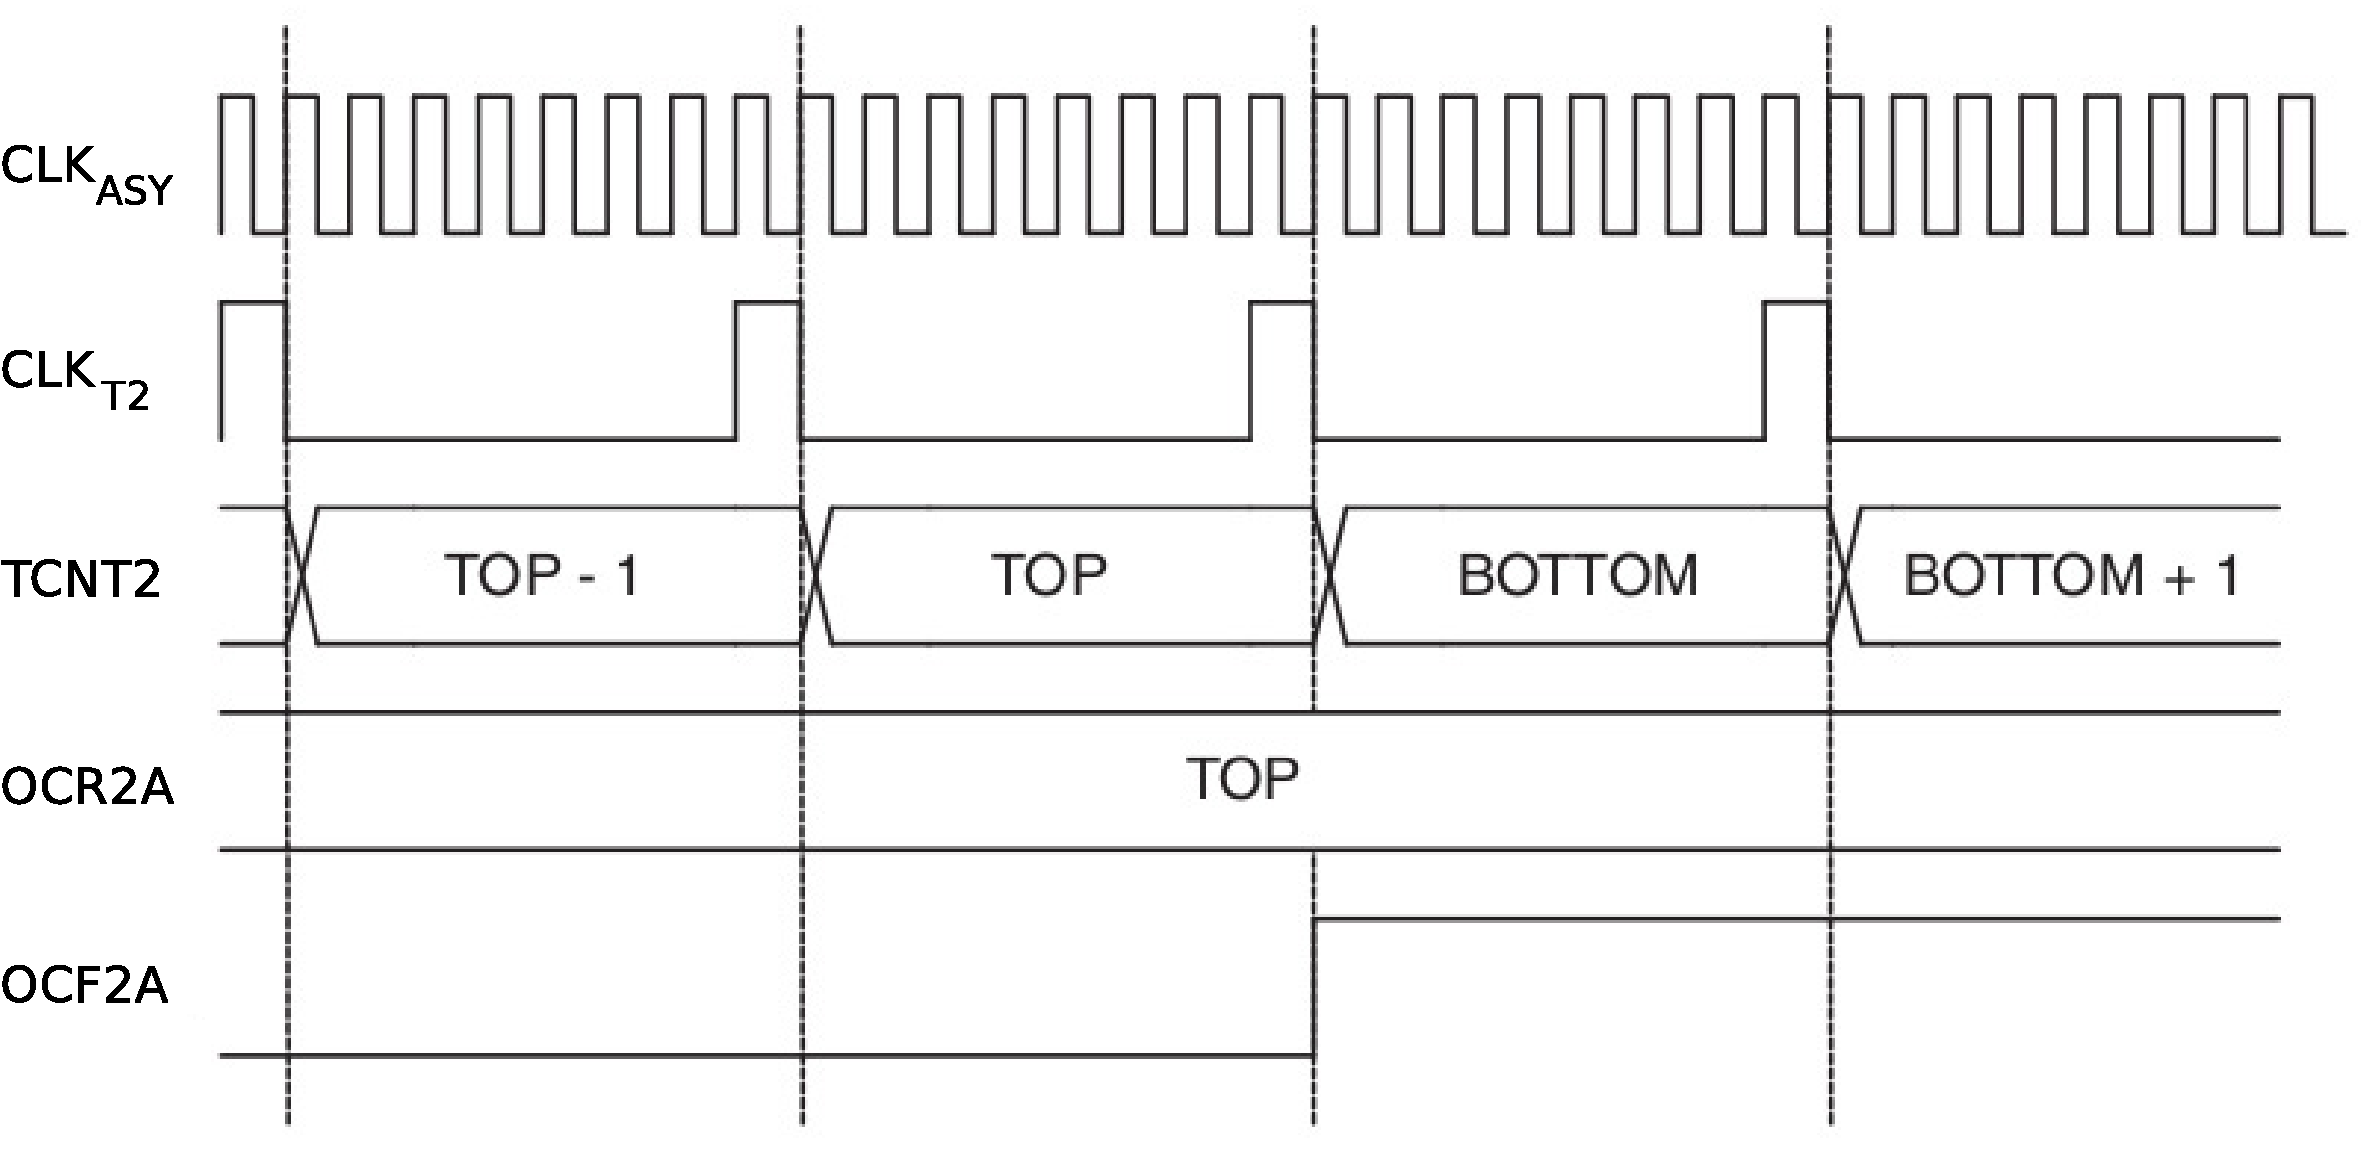
\includegraphics[width=12cm,keepaspectratio]{fig/timing-diagram.pdf}
  \caption{Timing diagram in CTC mode with prescaler 8 by Atmel Corporation}
  \label{fig:implementation-timing-diagram}
  \bigskip
\end{figure}

Additionally, when compare match occurs,
interrupt is raised and interrupt service routine {\it{AVR\_OUTPUT\_COMPARE\_INT}},
defined in {\it{cpu/avr/dev/clock.c}} file, is executed.
In this case is flag indicating occurred match {\it{OCF2A}}
cleared automatically by hardware when executing
the corresponding interrupt service routine~\cite{avr-datasheet}.

As described in section~\ref{sec:contiki-timers}, there is
{\it{CLOCK\_SECOND}} macro expressing number of clock interrupts per second.
To obtain {\it{CLOCK\_SECOND}} interrupts per second, there must be
${\frac{f_{T2}}{CLOCK\_SECOND}}$ hardware clock ticks between two successive interrupts.
On compare match in CTC mode, the timer is reset to zero as
shown on figure~\ref{fig:implementation-timing-diagram}.
The value zero is also included in the counting - the 0th count of the timer also takes one tick.
Therefore the value of compare register {\it{OCR2A}} must be ${\frac{f_{T2}}{CLOCK\_SECOND}} - 1$
when using Timer/Counter~2 in CTC mode.
Default value of {\it{CLOCK\_SECOND}} for AVR Raven in Contiki is 128,
what implies default value of compare register ${\frac{4096}{128}} - 1 = 31$.

The goal of interrupt service routine is to increment ...%! TODO as described in chapter??
% write to OCR2A
The interrupt service routine can be used for updating the value in compare register.
%However, changing TOP to a value close to BOTTOM when the counter is run-
%ning with none or a low prescaler value must be done with care since the CTC mode does not
%have the double buffering feature. If the new value written to OCR2A is lower than the current
%value of TCNT2, the counter will miss the compare match.

Adjusting time - CLOCK\_COMPARE\_REGISTER = 31 => 128Hz => 1s = 1s
FREQ = 32768/8 / 32
CLOCK\_COMPARE\_REGISTER = 30 => ca132.129Hz => 1s = ca1.032258s
FREQ = 32768/8 / 31
CLOCK\_COMPARE\_REGISTER = 32 => 124.12per => 1s = 0.96p
FREQ = 32768/8 / 33

=> fastest adjust is 0,03s / s

% READ - datasheet - 17.9. and 17.11.6 BUSY bit

This is enough for implementing a reasonable time interface and using it for NTP client later.

% ntp interface extending the clock library, similar to posix calls


Each TCNT2 increment is $\frac{1}{128 \times 32} \doteq 0,000244$ s
2,44ms minimum clock slew
This is also minimal possible clock adjustment.


Please note, that these adjustments will influence Contiki timers.
Applications requiring uninfluenced timers
are therefore advised to use rtimers, described in section~\ref{sec:contiki-timers},
because they use separate hardware clock unaffected by NTP client
(Timer/Counter~3 on AVR Raven platform).
